\documentclass[a4paper,12pt]{report}

\usepackage{cmap}
\usepackage[T2A]{fontenc}
\usepackage[utf8]{inputenc}
\usepackage[english,russian]{babel}
\usepackage{listings}
\usepackage{amsmath}
\usepackage{amsfonts}
\usepackage{float}
\usepackage{csquotes}
\usepackage{hyphenat}

% \usepackage{titlesec}
% \newcommand{\sectionbreak}{\clearpage}

\usepackage{graphicx}
\graphicspath{ {./images/} }

\usepackage{xcolor}
% \usepackage{courier}

\usepackage[
    backend=biber,
    style=alphabetic,
    sorting=ynt
]{biblatex}
\addbibresource{resources.bib}

\definecolor{buzzlightyear}{HTML}{8757A5}
\definecolor{grass}{HTML}{738D06}
\definecolor{sand}{HTML}{F18A2B}
\definecolor{comment}{HTML}{8E908B}

\lstdefinestyle{habrstyle}{
    backgroundcolor=\color{white},   
    commentstyle=\color{comment},
    keywordstyle=\bfseries\color{buzzlightyear},
    numberstyle=\tiny\color{comment},
    stringstyle=\color{grass},
    basicstyle=\ttfamily\footnotesize,
    breakatwhitespace=false,         
    breaklines=true,                 
    captionpos=b,                    
    keepspaces=true,                 
    numbers=left,                    
    numbersep=5pt,                  
    showspaces=false,                
    showstringspaces=false,
    showtabs=false,                  
    tabsize=4
}

\lstset{style=habrstyle}

\author{Луняк Николай}
\title{Лабораторная работа 5}
\date{\today}

\begin{document}
    \maketitle
    \tableofcontents
    \listoffigures
    \lstlistoflistings
    
    \chapter{Подбор высоты}
    
    В этом задании надо воспользоваться готовым материалом из \sloppy{\texttt{chap05.ipynb}} и, двигая слайдеры, подобрать период сигнала на основе автокорреляции.
    
    Будем последовательно выставлять разные значения для \texttt{start}, а затем, начиная с \texttt{offset} $=$ 0, подбирать период.
    
    Так как на слайдере не удается различить столь малые числа (а как настроить его по-другому мне не особо хочется разбираться), текущее значение \texttt{offset} буду запрашивать в отдельной ячейке как \texttt{slider1.value}.

    \begin{figure}[H]
        \centering
        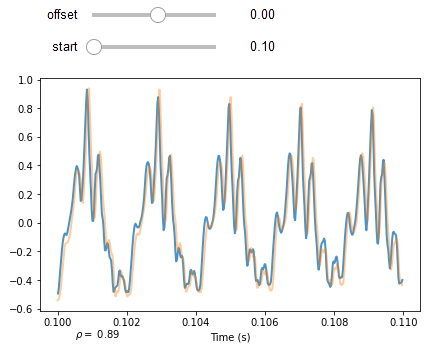
\includegraphics[width=0.75\textwidth]{ex1_21.png}
        \caption{Для \texttt{offset} $=$ 0.0021}
        \label{fig:ex1_21}
    \end{figure}
    
    \begin{figure}[H]
        \centering
        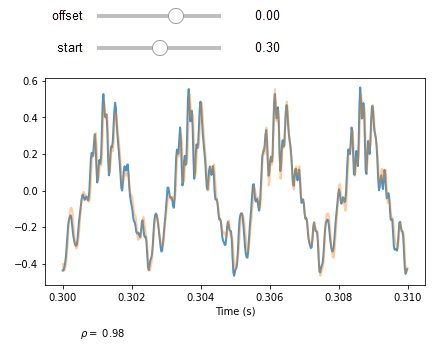
\includegraphics[width=0.75\textwidth]{ex1_25.png}
        \caption{Для \texttt{offset} $=$ 0.0025}
        \label{fig:ex1_25}
    \end{figure}
    
    \begin{figure}[H]
        \centering
        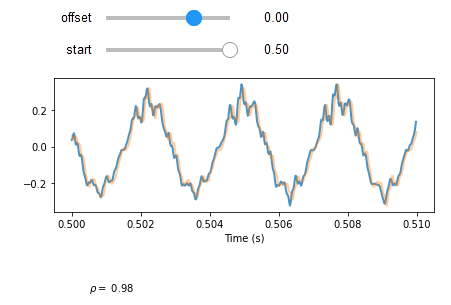
\includegraphics[width=0.75\textwidth]{ex1_28.png}
        \caption{Для \texttt{offset} $=$ 0.0028}
        \label{fig:ex1_28}
    \end{figure}
    
    Как мы можем видеть, \texttt{offset} меняется нелинейно, что логично, учитывая особенности исследуемого сигнала.
    
    \chapter{Автоматизируем процесс}
    
\begin{lstlisting}[language=Python,caption=Берем готовый код и загружаем звук]
from thinkdsp import Signal, Sinusoid, SquareSignal, TriangleSignal, SawtoothSignal, ParabolicSignal
from thinkdsp import normalize, unbias, PI2, decorate
from thinkdsp import Chirp
from thinkdsp import read_wave
from thinkdsp import Spectrum, Wave

import numpy as np
import pandas as pd

from matplotlib import pyplot

import thinkstats2

def serial_corr(wave, lag=1):
    """Computes serial correlation with given lag.

    wave: Wave
    lag: integer, how much to shift the wave

    returns: float correlation coefficient
    """
    n = len(wave)
    y1 = wave.ys[lag:]
    y2 = wave.ys[:n-lag]
    corr_mat = np.corrcoef(y1, y2)
    return corr_mat[0, 1]

def autocorr(wave):
    """Computes and plots the autocorrelation function.

    wave: Wave
    """
    lags = np.arange(len(wave.ys)//2)
    corrs = [serial_corr(wave, lag) for lag in lags]
    return lags, corrs

wave = read_wave('Sounds/28042__bcjordan__voicedownbew.wav')
wave.normalize()
wave.make_audio()
\end{lstlisting}

    Теперь реализуем функцию \texttt{estimate\_fundamental()} и сравним ее результат со спектрограммой (будем вызывать ее периодически, а потом соединим эти результаты одной линией поверх спектрограммы).
    
\begin{lstlisting}[language=Python,caption=Сравниваем]
def estimate_fundamental(segment, start=70, end=150):
    lags, correlations = autocorr(segment)
    lag = np.array(correlations[start:end]).argmax() + start
    period = lag / segment.framerate
    return 1 / period

ts = []
frequencies = []

for it in np.arange(0.0, 1.4, 0.05):
    ts.append(it + 0.025)
    segment = wave.segment(start=it, duration=0.01)
    frequency = estimate_fundamental(segment)
    frequencies.append(frequency)

wave.make_spectrogram(2048).plot(high=2000)
pyplot.plot(ts, frequencies, color='blue')
decorate(
    xlabel='Time (s)',
    ylabel='Frequency (Hz)'
)
\end{lstlisting}

    \begin{figure}[H]
        \centering
        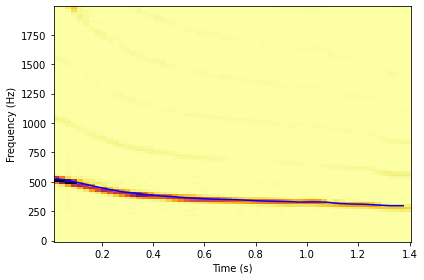
\includegraphics[width=0.75\textwidth]{images/ex2_comparison.png}
        \caption{Спектрограмма}
        \label{fig:ex2_comparison}
    \end{figure}
    
    Синяя линия ложится ровно поверх красной (основной частоты), что дает понять, что наше вычисление работает правильно.
    
    \chapter{Без BinCoin'а уже никуда}
    
    Загрузка данных аналогична прошлой лабораторной работе.
    
\begin{lstlisting}[language=Python,caption=Загрузка датасета]
data = pd.read_csv('Data/BTC_USD_2020-12-31_2021-03-30-CoinDesk.csv')
wave = Wave(data['Closing Price (USD)'], data.index, framerate=1)
wave.plot()
\end{lstlisting}

    \begin{figure}[H]
        \centering
        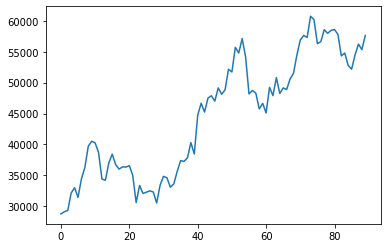
\includegraphics[width=0.75\textwidth]{images/ex3_wave.png}
        \caption{Курс битка}
        \label{fig:ex3_wave}
    \end{figure}
    
\begin{lstlisting}[language=Python,caption=Автокорреляция]
lags, correlations = autocorr(wave)
pyplot.plot(lags, correlations)
decorate(
    xlabel='Lag',
    ylabel='Correlation'
)
\end{lstlisting}

    \begin{figure}[H]
        \centering
        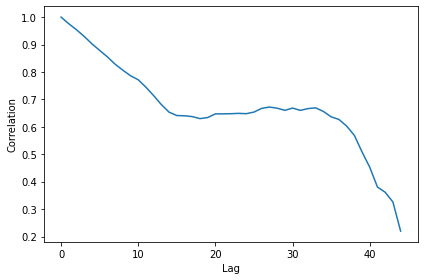
\includegraphics[width=0.75\textwidth]{images/ex3_autocorr.png}
        \caption{Автокорреляция}
        \label{fig:ex3_autocorr}
    \end{figure}
    
    Спадает она не быстро, больше походит на \textquote{розовый} шум, что согласуется с результатом предыдущей лабораторной работы.
    
    \chapter{Исследуем \texttt{saxophone.ipynb}}
    
    В рамках данного раздела нам предложен к рассмотрению файл \texttt{saxophone.ipynb}, в котором рассматривается феномент \textquote{отсутствующего основного тона}. От нас же требуется потыкать разные кнопки и посмотреть на разные результаты при выборе разных сегментов. И YouTube \cite{video} посмотреть еще.
    
    \begin{figure}[H]
        \centering
        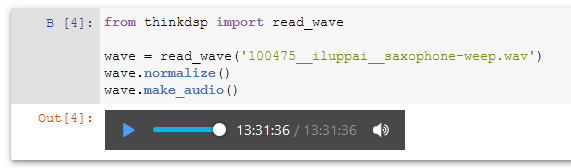
\includegraphics[width=0.75\textwidth]{images/ex4_original.png}
        \caption{KPACUBO}
        \label{fig:ex4_original}
    \end{figure}
    
    Если мы посмотрим на спектр участка $[2;2.5]$ секунд, то увидим следующую картину.
    
    \begin{figure}[H]
        \centering
        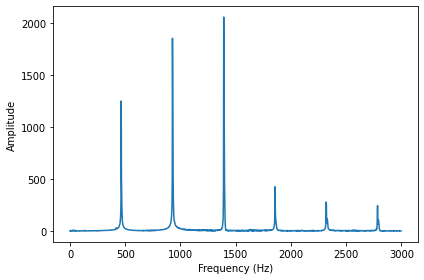
\includegraphics[width=0.75\textwidth]{images/ex4_spectrum_2s.png}
        \caption{Спектр вблизи 2 сек.}
        \label{fig:ex4_spectrum_2s}
    \end{figure}
    
    Хотя основной частотой и воспринимается 464 Гц, на самом деле ей должна была бы быть 1392 Гц. Объяснить этот эффект может помочь автокорреляция.
    
    \begin{figure}[H]
        \centering
        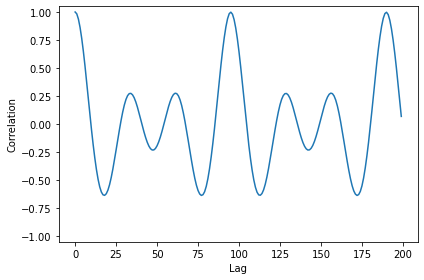
\includegraphics[width=0.75\textwidth]{images/ex4_autocorr.png}
        \caption{Автокорреляция}
        \label{fig:ex4_autocorr}
    \end{figure}
    
    Первый большой пик расположен вблизи 100 лага. Для того, чтобы вычислить точный лаг и соответствующую частоту, автор прибегает к коду, аналогичному \texttt{estimate\_fundamential()}. В итоге получается $(95, 464\text{Hz})$.
    
    Если удалить компоненту 464 Гц из спектра, то на слух все равно будет казаться, что основной тон 464 Гц. Этот эффект и называется \textquote{пропавшей} основной частотой (ладно, признаюсь, я читал оригинал ThinkDSP, а как по-русски это называется, я не знаю).
    
    Если снова нарисовать функцию автокорреляции, то окажется, что она совпадает с той, что мы видели ранее. Впрочем, на этом рисунке есть и другие пики, поменьше. Почему ухо воспринимает именно 464 Гц как основной тон? Оказывается, все остальные компоненты спектра - это гармоники 464 Гц, и именно на эту информацию опирается мозг при попытке оценить \textquote{настоящую} основную частоту.
    
    Если избавиться от гармоник (\texttt{high\_pass(600)}, \texttt{low\_pass(1200)}), то и сам эффект пропадает.
    
    Видео, кстати, тоже интересное.
    
    \printbibliography
    
\end{document}
